% Na zvoleném českém korpusu vyhodnoťte přesnost a pokrytí pravidel. Diskutujte míru, se kterou je možné generovat gramatické věty, a kvalitu textu (přirozené vyjadřování, nezamýšlené vedlejší efekty).

\section{Evaluation Corpus}

For evaluation, I have constructed my own text corpus. The corpus is composed of texts written by contemporary Czech authors who provided the texts themselves for this purpose. The corpus is intentionally small as the evaluation was done by humans, and evaluation of a large set of sentences would be expensive.

In selecting the texts, I tried to capture various characteristics of the texts. Thus, the corpus consists of several different literary genres, the narrators are both male and female, I have included texts written in the present and past tense, and I have chosen texts containing different types of speech. (Such as direct speech, semi-direct speech...) Finally, the corpus of course includes both first-person and third-person narratives.

In total, the evaluation data consists of 36 different texts composed of 388 sentences. The numbers divided by narratives are captured in chart \ref{fig:eval-input-numbers}.

\begin{figure}[!ht]
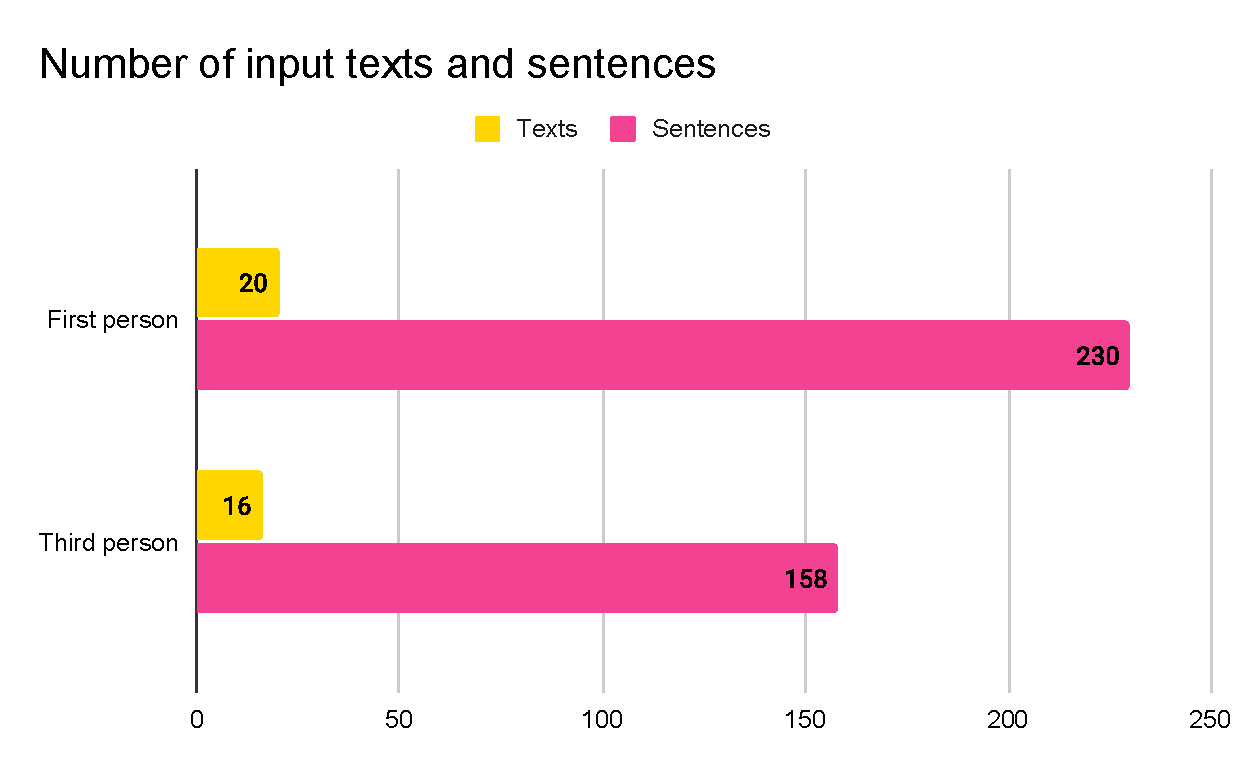
\includegraphics[width=\textwidth]{data/Eval-Input-Numbers.pdf}
\caption{Statistics about the corpus}
\label{fig:eval-input-numbers}
\end{figure}

\section{Annotation Process}

As mentioned in previous section, the sentences were evaluated manually by human annotators. The annotators have got: the person which the text be converted from, the name of the protagonist, the original text, and the rephrased text. After reading the texts, an annotator could mark one or more statements for each sentence as true.

The possible statements to mark:

\begin{itemize}
	\item The sentence is converted correctly, without grammatical errors, sounds natural and it is unambiguous in meaning.
	\item The sentence has lost its unambiguity.
	\item The word order is unnatural, or there are other unnatural sounding elements in the sentence.
	\item The sentence contains grammatical errors.
	\item Some parts of the sentence are converted correctly, and some are not.
	\item The sentence is not converted correctly or not converted at all.
	\item The sentence has not been converted in any way, and that is correct.
\end{itemize}

The evaluation's non-binarity also offers a basic error analysis, which gives us a basis for discussion about the quality of generated texts.

\section{Results}

Based on the marking, I retrieved the results statistics.

As can be seen in figure \ref{fig:eval-total}, most of the sentences were converted correctly, that also includes not converting the sentence at all (about 66\%). Only 17\% of the 388 sentences were coverted incorrecly, partially or completely. The remaining 17\% are sentences which were converted correctly, however, the conversion damaged the text's quality, such as naturality of expression, unambiguity or grammar.

\begin{figure}[!ht]
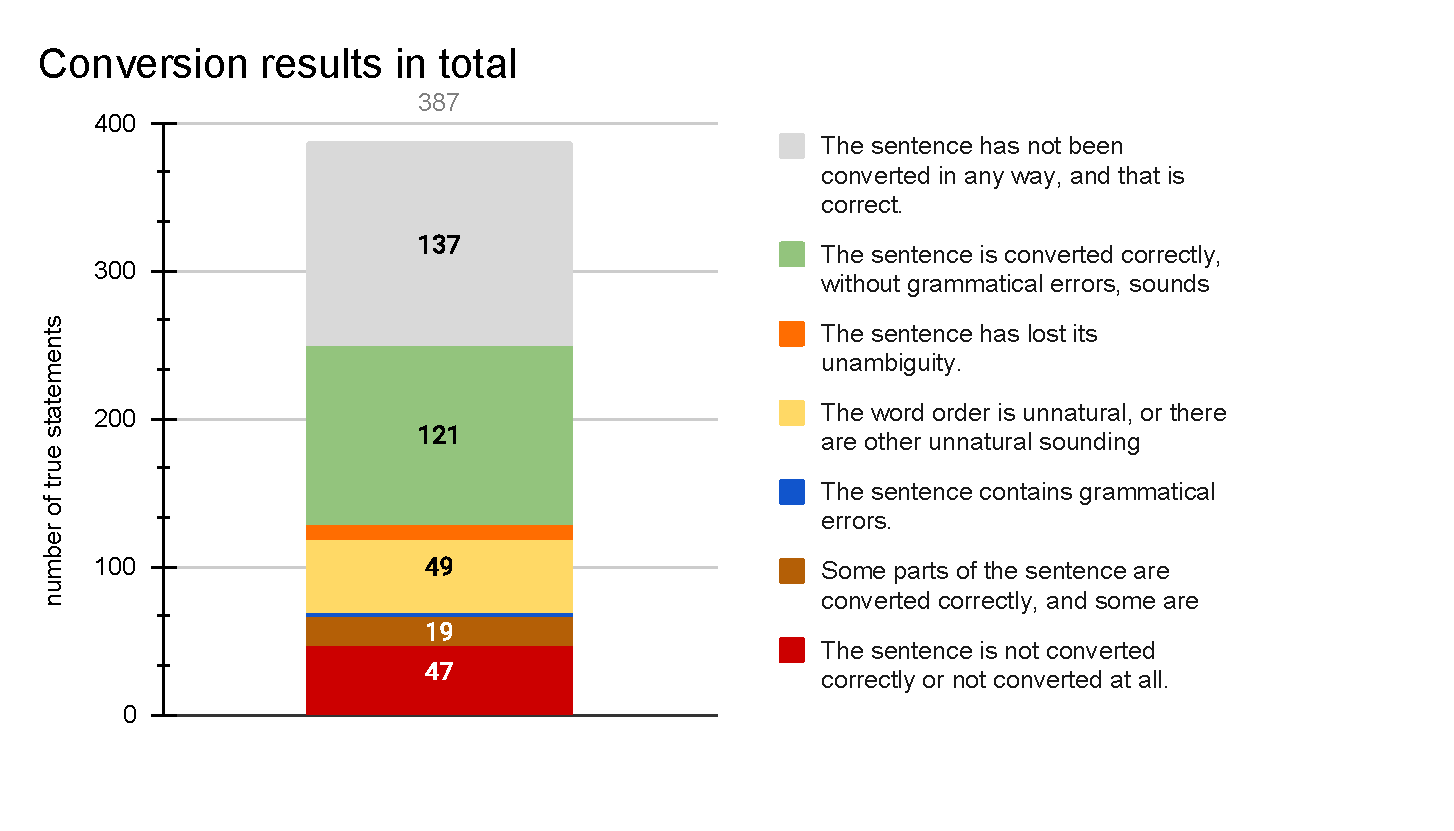
\includegraphics[width=\textwidth]{data/Eval-Total.pdf}
\caption{Results statistics in total}
\label{fig:eval-total}
\end{figure}

Now let's take a look at the results for each narrative mode.

\subsection{First-person to Third-person results}

\ref{fig:eval-first-to-third}

\begin{figure}[!ht]
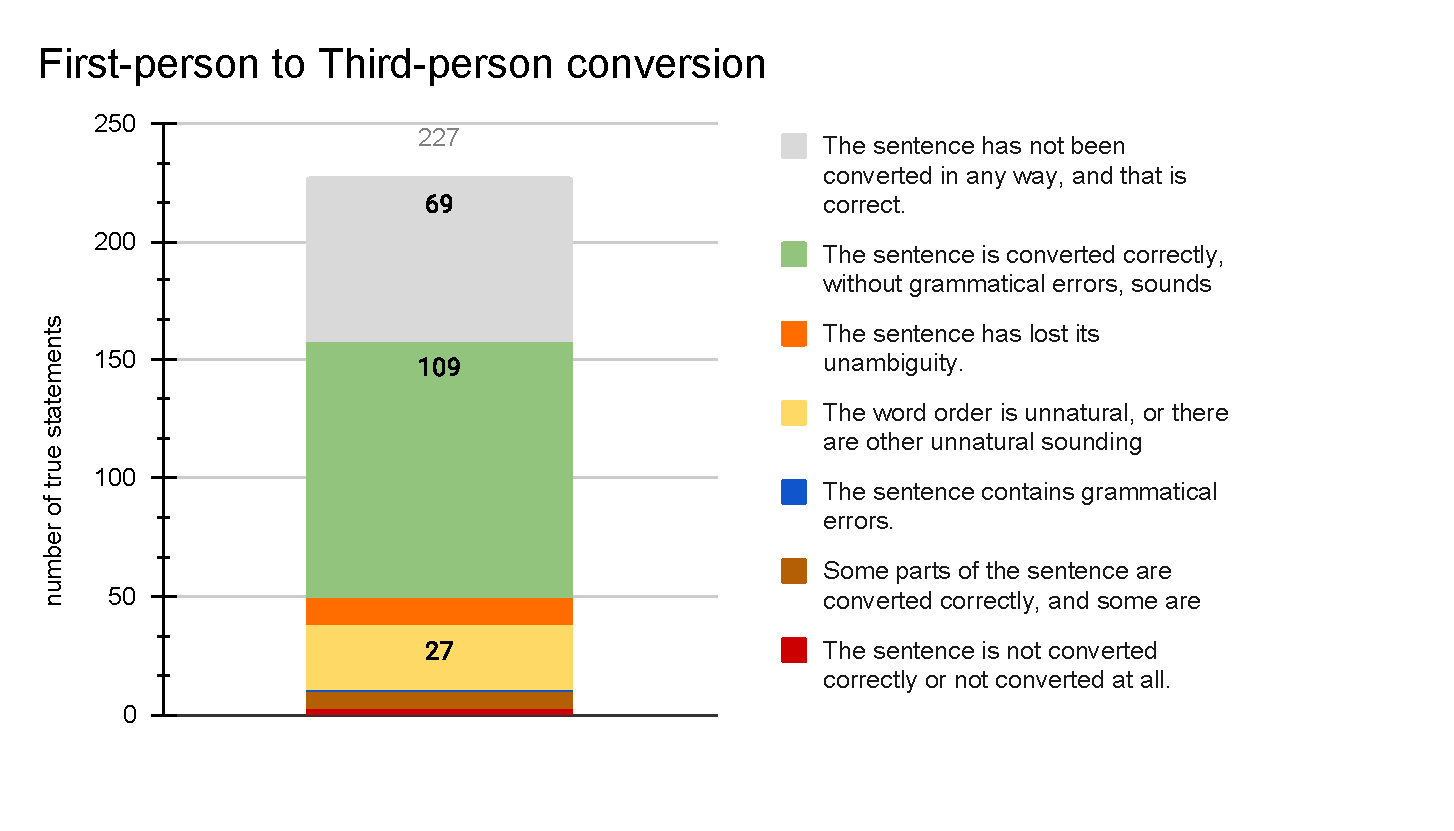
\includegraphics[width=\textwidth]{data/Eval-First-To-Third.pdf}
\caption{Results statistics for first-person to third-person conversion}
\label{fig:eval-first-to-third}
\end{figure}

\subsection{Third-person to First-person results}
\ref{fig:eval-third-to-first}

\begin{figure}[!ht]
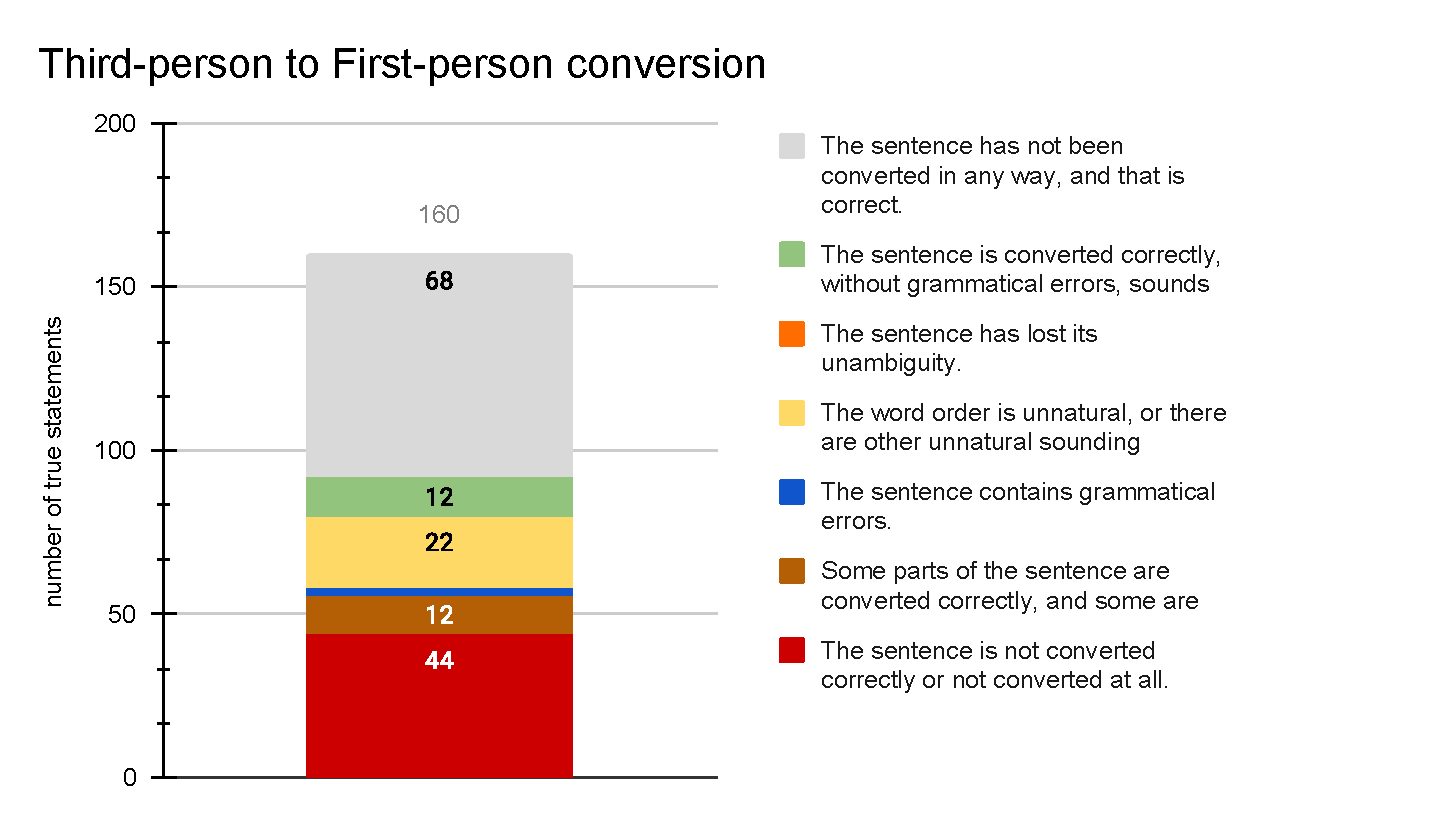
\includegraphics[width=\textwidth]{data/Eval-Third-To-First.pdf}
\caption{Results statistics for third-person to first-person conversion}
\label{fig:eval-third-to-first}
\end{figure}

